\documentclass[12pt]{article}

\usepackage{graphicx}
\usepackage{vhistory}
\usepackage{amsfonts}
\usepackage{amsmath}
\usepackage{hhline}
\usepackage{booktabs}
\usepackage{url}

\oddsidemargin 0mm
\evensidemargin 0mm
\textwidth 160mm
\textheight 200mm
\renewcommand\baselinestretch{1.0}

\pagestyle {plain}
\pagenumbering{arabic}

\newcounter{stepnum}

%% Comments


\begin{document}

\title{\textbf{LiveLong}}
\author{Version 1.4\\ \\CS 2XB3 \\ Computer Science Practice and Experience: Binding Theory to Practice
\\ Lab Section: L02\\Group: 08\\ \\Kenneth Mak - 001318946}
\date{April 12, 2020}

\maketitle
\newpage
\begin{versionhistory}
\vhEntry{1.0}{08.04.2020}{KM}{Document created}
\vhEntry{1.1}{09.04.2020}{KM}{Figures added}
\vhEntry{1.2}{09.04.2020}{KM}{Description of implementation added, edits to figures}
\vhEntry{1.3}{11.04.2020}{KM}{Added Internal Review of design, edits to phrasing in other areas}
\vhEntry{1.4}{12.04.2020}{KM}{Document finalized}
\end{versionhistory} 
\bigskip
\textit{By virtue of submitting this document we electronically sign and date that the work being submitted by all the individuals in the group is their exclusive work as a group and we consent to make available the application developed through CS-2XB3 project, the reports, presentations, and assignments (not including my name and student number) for future teaching purposes.}

%%%%%%%%%%%%%%%%%%%%%%%%%%%%%%%% TABLE OF CONTENTS
\newpage
\tableofcontents
%%%%%%%%%%%%%%%%%%%%%%%%%%%%%%%% TABLE OF CONTENTS
%%%%%%%%%%%%%%%%%%%%%%%%%%%%%%%%
\newpage
\section{Contributions}
As this project was completed by a single member, the Role column is deemed unnecessary. Instead the contributions will list the amount of work completed.

\begin{center}
\begin{tabular}{|p{0.2\hsize}|p{0.75\hsize}|}
\hline
\textbf{Name} & \textbf{Contributions}\\
\hline
Kenneth Mak & Research of Valid Projects\\
  & Wrote Project Proposal\\
  & Project Presentation\\
  & Wrote Requirements Specifications\\
  & Designed and implemented DataReader class to read from CSV files\\
  & Implemented DataWriter class to write object data to CSV files\\
  & Geocoded the locations of all NursingHomes into a dataset\\
  & NursingHome ADT\\
  & NHGeoInfo ADT\\
  & Deficiency ADT\\
  & Implementation of longitude-latitude distance calculations\\
  & Implementation of geocoding an address during runtime using OSM\\
  & Implemented ability to change user location during runtime\\
  & Implementation of QuickSort algorithm for arrays and lists\\
  & Implementation of Sequential Search Symbol Table\\
  & Implementation of Separate-Chaining Hash Table for efficient Sort algorithms\\
  & Added sorting order to NursingHome and NHGeoInfo ADT\\
  & Implemention of search filter to return list of objects from the database\\
  & Created interactive menu with the command line interface\\
  & Wrote TextParser to respond to commands\\
  & Implemented Application run-loop and basic logic\\
  & Designed text UI and viewer\\
  & Implemented ability to open GoogleMaps on desktop browser\\
  & Handled errors and bugs\\
  & Wrote documents and specifications\\
\hline
\end{tabular}
\end{center}




%%%%%%%%%%%%%%%%%%%%%%%%%%%%%%%% ABSTRACT
\newpage
\section{Executive Summary}
LiveLong is an application that quickly and accurately delivers information about nursing homes in the U.S. with official government datasets provided by Medicare. Clients can quickly search through the official datasets to get a quick and informed look at prospective nursing homes. Clients may modify a search filter to get better results that fulfil their requirements, such as selecting nursing homes that are ‘Special Focus’, or only selecting nursing homes with a rating over 3. \\ \\
Results are presented based on overall ratings and distance to the client. The ratings of each nursing home are conducted with current and previous residents. These ratings include areas concerning long-term and short-term stay experiences, the quality of the services, and the quality of the staff.
\\ \\
The application also highlights any warnings and active deficiencies the nursing home has, such as having a history of abuse cases. Active deficiencies, should there be any, will notify the clients of its severity and the duration of when it was first assigned, and whether it has been resolved or not.
%%%%%%%%%%%%%%%%%%%%%%%%%%%%%%%% ABSTRACT
%%%%%%%%%%%%%%%%%%%%%%%%%%%%%%%%%%		Overview
\newpage
\section{Module and Class Overview}

\subsection{Module Decomposition}

The application was implemented with a Model-View-Controller design pattern. The application is separated into four different packages.
\begin{enumerate}
\item \textbf{classes} - Contains all ADT classes
\item \textbf{data} - The Model, database and file parsing classes
\item \textbf{app} - The Main application, View and Controller classes
\item \textbf{util} - Utilities module providing access to data structures, algorithms, and access to OSM \& GoogleMaps functionalities
\end{enumerate}

\noindent Refer to Figure \ref{fig:ClassUML} for visual representation of classes and their relationships.

\subsubsection{classes package}
Classes placed in here are used to store information parsed from a Dataset into an object.
\begin{itemize}
\item \textbf{NursingHome.java} ADT stores information about a Nursing Home. Each NursingHome has a unique ID
\item \textbf{NHGeoInfo.java} ADT stores geographical information about a Nursing Home. Corresponds to the NursingHome object with the same ID.
\item \textbf{NHPair.java} ADT stores a corresponding \textbf{NursingHome} and \textbf{NHGeoInfo}. Used for passing search results
\item \textbf{Deficiency.java} ADT stores information about a Deficiency that was assigned to a NursingHome. Refers to a specific NursingHome by ID.
\item \textbf{FireSafetyDeficiency.java} ADT is a subclass of Deficiency
\item \textbf{HealthDeficiency.java} ADT is a subclass of Deficiency
\end{itemize}

\subsubsection{data package}
Classes are used to parse information from CSV files and store them in memory to be interacted with. It also provides the ability to write compressed CSV files to be used for initialization instead of the original datasets, reducing initialization times.
\begin{itemize}
\item \textbf{Database.java} is the Model of the MVC design pattern. All ADTs from classes constructed from parsed datasets are stored here.
\item \textbf{DataReader.java} is used to read information from datasets and construct the appropriate ADTs
\item \textbf{DataWriter.java} is used to write ADT information into a CSV format such that the same ADTs can be constructed with the CSV
\end{itemize}


\subsubsection{app package}
Classes placed in here are used to parse user response and pull information from the Database, which is located in the \textbf{data} package.
\begin{itemize}
\item \textbf{LiveLong.java} is the main application loop
\item \textbf{Controller.java} is used to send requests to the Database and receive the result of searches. Passes results to \textbf{TextParser}
\item \textbf{TextParser} is the View of the MVC pattern. Displays the UI in the command line and parses user response into commands for the Controller to send.
\item \textbf{State.java} is an enum denoting the current state of the application (I.e. Menu, Settings, Exiting, etc.)
\end{itemize}

\subsubsection{util package}
Classes here provide common utility functions, algorithms, or data structures to be used by other classes. Not specific to this LiveLong application.
\begin{itemize}
\item \textbf{GoogleMapUtils.java} provides a method to open GoogleMaps in desktop browser with an origin and destination
\item \textbf{OpenStreetMapUtils.java} provides a method to return the geocoded location details of an address
\item \textbf{QuickSort.java} provides QuickSort algorithm implementation for arrays and lists
\item \textbf{SeparateChainingHashST.java} provides a HashTable for efficient insert and search operations. Uses SequentialSearchST.
\item \textbf{SequentialSearchST.java} provides a SymbolTable list for quick insert and search operations.
\end{itemize}
Both \textbf{SequentialChainingHashST} and \textbf{SequentialSearchST} were created from Lab 9 of CS2XB3.

\begin{center}
\begin{figure}
\includegraphics[width=16cm]{Pictures/uml.png}
\caption{UML Class diagram showing a static representation of LiveLong application classes and relationships}
\label{fig:ClassUML}
\end{figure}
\end{center}

\subsubsection{Explanation}
The usage of an MVC design pattern enforces the Separation of Concerns design principle. Changes to one module or class should not affect another module that they both needed be modified. This allows for faster and more efficient modifications to the application to be carried out in the future.
\\ \\
For example, as a possible change, say the application needs to change from a CLI program to a visual GUI. The developer would not need to make changes to how the Database or Controller modules work. All they would have to do is develop a new class to be used in place of TextParser to act as the View of the MVC design pattern. This new class would instead generate a GUI, but still send parsed user interactions to the unchanged Controller module.
\\ \\
Other possible changes could include how CSV files may have their structure changed, or if better algorithms need to be implemented to account for scalability. These changes can then be fixed by only modifying their specific code in \textbf{DataReader} and in \textbf{SequentialSearchHashST}
%%%%%%%%%%
\newpage
\subsection{Classes Package Overview}

\subsubsection{NursingHome ADT}
\begin{center}
\begin{tabular}{p{0.1\hsize}|p{0.25\hsize}|p{0.50\hsize}}
\multicolumn{3}{l}{\textbf{public class NursingHome}} \\
\hline
 & NursingHome(String[]) & Constructs an immutable NursingHome object from a String array, usually parsed from the CSV file\\
\hline
String 	& getID() & Returns the ID of this NursingHome\\
\hline
String 	& getAddress() & Returns the Address of this NursingHome\\
\hline
void 		& addDef() & Adds a Deficiency to this NursingHome \\
\hline
int 		& getActiveDefCount() & Counts the number of active deficiencies \\
\hline
int 		& getOverallRating() & Gets the overall rating \\
\hline
String	& getSFF() & Gets the Special Focus status \\
\hline
boolean 	& getAbuse() & Returns Abuse variable \\
\hline
boolean 	& getOldSurvey() & Returns OldSurvey variable\\
\hline
String 	& toString() & Returns a String showing only the important values\\
\hline
String 	& detailed() & Returns a String with all the values \\
\hline
String[] 	& toCSV() & Returns all values in state variables\\
\hline
\end{tabular}
\end{center}

\subsubsection{NHGeoInfo ADT}
\begin{center}
\begin{tabular}{p{0.1\hsize}|p{0.25\hsize}|p{0.50\hsize}}
\multicolumn{3}{l}{\textbf{public class NHGeoInfo}} \\
\hline
 & NHGeoInfo(String[]) & Constructs a NHGeoInfo object from a String array, usually parsed from the CSV file\\
\hline
void 	& calculateDistance ($lat2$, $lon2$) & Calculates and sets the distance value of this object to the distance between this latitude and longitude with target $lat2$ and $lon2$\\
\hline
String 	& getID() & Returns the NursingHome ID that this NHGeoInfo refers to\\
\hline
double 	& getLatitude() & Returns the latitude value\\
\hline
double 	& getLongitude() & Returns the longitude value \\
\hline
double 	& getDistance() & Returns the distance between this object and a target location \\
\hline
String[] 	& toCSV() & Returns all values in state variables\\
\hline
\end{tabular}
\end{center}


\subsubsection{NHPair ADT}
\begin{center}
\begin{tabular}{p{0.18\hsize}|p{0.17\hsize}|p{0.50\hsize}}
\multicolumn{3}{l}{\textbf{public class NHPair}} \\
\hline
 & NHPair (NursingHome, NHGeoInfo) & Constructs a NHPair object with the two objects, such that both their IDs are the same \\
\hline
NursingHome 	& getLeft() & Returns the NursingHome object\\
\hline
NHGeoInfo		& getRight() & Returns the NHGeoInfo object\\
\hline
\end{tabular}
\end{center}

\bigskip
\subsubsection{Deficiency ADT}
\begin{center}
\begin{tabular}{p{0.1\hsize}|p{0.25\hsize}|p{0.50\hsize}}
\multicolumn{3}{l}{\textbf{public class Deficiency}} \\
\hline
 & Deficiency(String[]) & Constructs an immutable Deficiency object from a String array, usually parsed from the CSV file\\
\hline
boolean 	& isActive() & Check the status of deficiency and the status date \\
\hline
String 	& getID() & Returns the NursingHome ID that this Deficiency refers to\\
\hline
String 	& getDefStartDate() & Returns when this deficiency was assigned\\
\hline
String 	& getDefCategory() & Returns the category of this deficiency\\
\hline
String 	& getDefDescription() & Returns the description of this deficiency\\
\hline
String 	& getDefStatus() & Returns the status of this deficiency\\
\hline
String 	& getDefStatusDate() & Returns the date of when the status changed\\
\hline
String[] 	& toCSV() & Returns all values in state variables\\
\hline
\end{tabular}
\end{center}

\newpage

\subsubsection{FireSafetyDeficiency ADT}
\begin{center}
\begin{tabular}{p{0.1\hsize}|p{0.25\hsize}|p{0.50\hsize}}
\multicolumn{3}{l}{\textbf{public class FireSafetyDeficiency extends Deficiency}} \\
\hline
 & FireSafetyDeficiency (String[]) & Constructs an immutable FireSafetyDeficiency object from a String array, usually parsed from the CSV file\\
\hline
String	& toString() & Returns a string detailing this Fire Safety Deficiency\\
\hline
\end{tabular}
\end{center}

\bigskip

\subsubsection{HealthDeficiency ADT}
\begin{center}
\begin{tabular}{p{0.1\hsize}|p{0.25\hsize}|p{0.50\hsize}}
\multicolumn{3}{l}{\textbf{public class HealthDeficiency extends Deficiency}} \\
\hline
 & HealthDeficiency (String[]) & Constructs an immutable HealthDeficiency object from a String array, usually parsed from the CSV file\\
\hline
String	& toString() & Returns a string detailing this Health Deficiency\\
\hline
\end{tabular}
\end{center}
%%%%%%%%%%%%%%%%%%%%

\newpage
\subsection{Data Package Overview}
\subsubsection{Database}
\begin{center}
\begin{tabular}{p{0.1\hsize}|p{0.25\hsize}|p{0.50\hsize}}
\multicolumn{3}{l}{\textbf{public class Database}} \\
\hline
 & Database (String) & Sets user location to string and get geocode of location. Parses the information from the dataset into data structures with DataReader. NursingHome objects are placed into a Hash table. Deficiencies are added to the corresponding NursingHome object by ID. NHGeoInfo objects have their distance values recalculated to the user location.\\
\hline
void 	& ChangeLocation (String) & Attempts to change the user location to new parameter. If Geocoding the new address is successful, save new location and update all NHGeoInfo objects with new location. \\
\hline
seq of NHPair 	& search(int, int, bool, bool, ...) & Returns a list of NHPair objects with NursingHome objects that satisfy the search criteria in the parameters\\
\hline
double 	& getAddress() & Returns the address/user location\\
\hline
double 	& getLatitude() & Returns the latitude value of address\\
\hline
double 	& getLongitude() & Returns the longitude value of address \\
\hline
\end{tabular}
\end{center}

\newpage
\subsubsection{DataReader}
\begin{center}
\begin{tabular}{p{0.13\hsize}|p{0.25\hsize}|p{0.47\hsize}}
\multicolumn{3}{l}{\textbf{public class DataReader}} \\
\hline
static (seq of NursingHome) & getNursingHomeInfo() & Returns a list of NursingHome objects constructed from the CSV dataset\\
\hline
static (seq of NHGeoInfo) & getNHGeoInfo() & Returns a list of NHGeoInfo objects constructed from the CSV dataset\\
\hline
static (seq of FireSafetyDeficiency) & getFireSafetyInfo() & Returns a list of FireSafetyDeficiency objects constructed from the CSV dataset\\
\hline
static (seq of HealthDeficiency) & getHealthInfo() & Returns a list of HealthDeficiency objects constructed from the CSV dataset\\
\hline
\end{tabular}

\end{center}
\subsubsection{DataWriter}
\begin{center}
\begin{tabular}{p{0.13\hsize}|p{0.25\hsize}|p{0.47\hsize}}
\multicolumn{3}{l}{\textbf{public class DataWriter}} \\
\hline
static void & SaveNursingHomeInfo (seq of NursingHome) & Saves a list of NursingHome objects into a CSV\\
\hline
static void & SaveNHGeoInfo (seq of NHGeoInfo) & Saves a list of NHGeoInfo objects into a CSV\\
\hline
static void & SaveFireSafetyInfo (seq of FireSafetyDeficiency) & Saves a list of FireSafetyDeficiency objects into a CSV\\
\hline
static void & SaveHealthInfo (seq of HealthDeficiency) & Saves a list of HealthDeficiency objects into a CSV\\
\hline
\end{tabular}
\end{center}
%%%%%%%%%%%%%%%%%%%%

\newpage
\subsection{App Package Overview}
\subsubsection{LiveLong}
\begin{center}
\begin{tabular}{p{0.1\hsize}|p{0.25\hsize}|p{0.50\hsize}}
\multicolumn{3}{l}{\textbf{public class LiveLong}} \\
\hline
static void & main(String[]) & Initialize the \textbf{Database}, \textbf{Controller}, and \textbf{TextParser} classes. Set application state to \textit{State.Menu}. Start application loop. In each loop, request user input. Upon receiving user input, send to TextParser the response and current application state. End loop when application state changes to \textit{State.Exiting}. \\
\hline
static State 	& getAppState (String) & Returns the current application state \\
\hline
static void 	& setAppState (State) & Changes the application state to parameter. Prompts \textbf{TextParser} to printScreen(State) \\
\hline
\end{tabular}
\end{center}


\subsubsection{State enum}
\begin{center}
\begin{tabular}{p{0.20\hsize}p{0.7\hsize}}
\multicolumn{2}{l}{\textbf{public enum State}} \\
\hline
State Enum & ~ \\
\hline
Menu & While in Menu state, user can choose to start a search, go to Settings state, or exit \\
Settings & While in Settings state, user can choose to modify their search results and current location, or return to Menu state. \\
Searching & While in Searching state, application is requesting results from Database based on search filter. No user input allowed until Database finishes search \\
Finished & While in Finished state, results of search are shown on screen. User can choose to examine a result and open them in Google Maps. User can return to Menu state \\
Exiting & While in Exiting state, application is shutting down. No user input allowed. \\
\hline
\end{tabular}
\end{center}

\newpage
\subsubsection{Controller}
\begin{center}
\begin{tabular}{p{0.1\hsize}|p{0.25\hsize}|p{0.50\hsize}}
\multicolumn{3}{l}{\textbf{public class Controller}} \\
\hline
 & Controller (Database) & Initialize the \textbf{Controller} with a reference to the Database \\
\hline
void  	& sendSearch (int, int, bool, bool, ...) & Send parameters to db.search() function, and store the results in local variable\\
\hline
seq of NHPair  	& getResults() & Return the list of NHPair received after sendSearch() method \\
\hline
void & requestChangeLocation (String) & Send a prompt to Database to change locations \\
\hline
String & getAddress () & Get the current user location from the Database object \\
\hline
void & setNumResults(int) & Change search filter to return only x amount of results\\
\hline
int & getNumResults() & Get current maximum number of results \\
\hline
void & setMinRating(int) & Change search filter to return objects with rating over x\\
\hline
int & getMinRating() & Get current minimum rating in filter\\
\hline
void & setFilterForSFF (bool) & Change search filter SFF to bool\\
\hline
boolean & isFilterForSFF() & Return true if search filtering for SFF Nursing Homes\\
\hline
void & setFilterAbuse(bool) & Change search filter for Abuse flags to bool\\
\hline
boolean & isFilterAbuse() & Return true if search filtering out Abuse flags\\
\hline
void & setFilterOldSurvey (bool) & Change search filter for OldSurvey flags to bool\\
\hline
boolean & isFilterOldSurvey() & Return true if search filtering out OldSurvey flags\\
\hline
void & setSortByRank(bool) & Change if results should be sorted by ratings first\\
\hline
boolean & isSortByRank() & Return true if results are returned sorted by ratings first, then distance\\
\hline
\end{tabular}
\end{center}

\newpage
\subsubsection{TextParser}
\begin{center}
\begin{tabular}{p{0.1\hsize}|p{0.25\hsize}|p{0.50\hsize}}
\multicolumn{3}{l}{\textbf{public class TextParser}} \\
\hline
 & TextParser(Controller) & Initialize the \textbf{TextParser} with a reference to the Controller \\
\hline
void & receive(String, State) & Handle the String response of user based on the current State, and send parsed commands to Controller\\
\hline
void & printScreen(State) & Prints the screen corresponding to the given State in the command line\\
\hline
\end{tabular}
\end{center}


%%%%%%%%%%%%%%%%%%%%

\newpage
\subsection{Util Package Overview}
\subsubsection{GoogleMapsUtils}
\begin{center}
\begin{tabular}{p{0.15\hsize}|p{0.25\hsize}|p{0.45\hsize}}
\multicolumn{3}{l}{\textbf{public class GoogleMapsUtils}} \\
\hline
 & GoogleMapsUtils() & Create singleton instance of self \\
\hline
static GoogleMapsUtils & getInstance() & Returns the singleton instance \\
\hline
void 	& openMaps (String, String) & Opens GoogleMaps in default desktop browser with the origin and destination set to the provided locations \\
\hline
\end{tabular}
\end{center}

\bigskip

\subsubsection{OpenStreetMapUtils}
\begin{center}
\begin{tabular}{p{0.1\hsize}|p{0.25\hsize}|p{0.50\hsize}}
\multicolumn{3}{l}{\textbf{public class OpenStreetMapUtils}} \\
\hline
 & OpenStreetMapUtils() & Create singleton instance of self \\
\hline
static OpenStreetMapUtils & getInstance() & Returns the singleton instance \\
\hline
Map $\langle$String, double$\rangle$ & getCoordinates(String) & Attempts to geocode the given address and return the latitude and longitude \\
\hline
\end{tabular}
\end{center}

\bigskip
\subsubsection{QuickSort}
\begin{center}
\begin{tabular}{p{0.1\hsize}|p{0.25\hsize}|p{0.50\hsize}}
\multicolumn{3}{l}{\textbf{public class QuickSort}} \\
\hline
void & sort(T[ ]) & Sorts the given array using QuickSort \\
\hline
void & sort(List$<$T$>$) & Sorts the given list using QuickSort \\
\hline
\end{tabular}
\end{center}

\newpage
\noindent \textbf{SeparateChainingHashST} and \textbf{SequentialSearchST} classes are pulled from Lab 9 of CS2XB3.

\subsubsection{SeparateChainingHashST}
\begin{center}
\begin{tabular}{p{0.1\hsize}|p{0.35\hsize}|p{0.40\hsize}}
\multicolumn{3}{l}{\textbf{public class SeparateChainingHashST}} \\
\hline
& SeparateChainingHashST(int) & Constructs a hash table with size of int \\
\hline
Value & get(Key) & Searches for the Key in hash table, and returns the Value associated with it \\
\hline
void & put(Key, Value) & Inserts the Key and Value in hash table. If key exists, replace previous value with new Value \\
\hline
Iterable $<$Key$>$ & keys() & Returns the set of all keys in hash table \\
\hline
\end{tabular}
\end{center}


\bigskip


\subsubsection{SequentialSearchST}
\begin{center}
\begin{tabular}{p{0.1\hsize}|p{0.25\hsize}|p{0.50\hsize}}
\multicolumn{3}{l}{\textbf{public class SequentialSearchST}} \\
\hline
& SequentialSearchST() & Initializes an empty linked list of nodes\\
\hline
Value & get(Key) & Searches for the Key in linked list, and returns the Value associated with it \\
\hline
void & put(Key, Value) & Inserts the Key and Value in list. If key exists, replace previous value with new Value \\
\hline
void & delete(Key) & Removes the target Key and associated Value from list \\
\hline
boolean & contains(Key) & Return true if key is found in list \\
\hline
boolean & isEmpty() & Return true if size() is 0 \\
\hline
int & size() & Returns size of list \\
\hline
Iterable $<$Key$>$ & keys() & Returns the set of all keys in list \\
\hline
\end{tabular}
\end{center}

%%%%%%%%%%%%%%%%%%%%%%%%%%%%%%%%%%			USES RELATIONSHIP
\newpage
\section{View of the Uses relationship}

\begin{center}
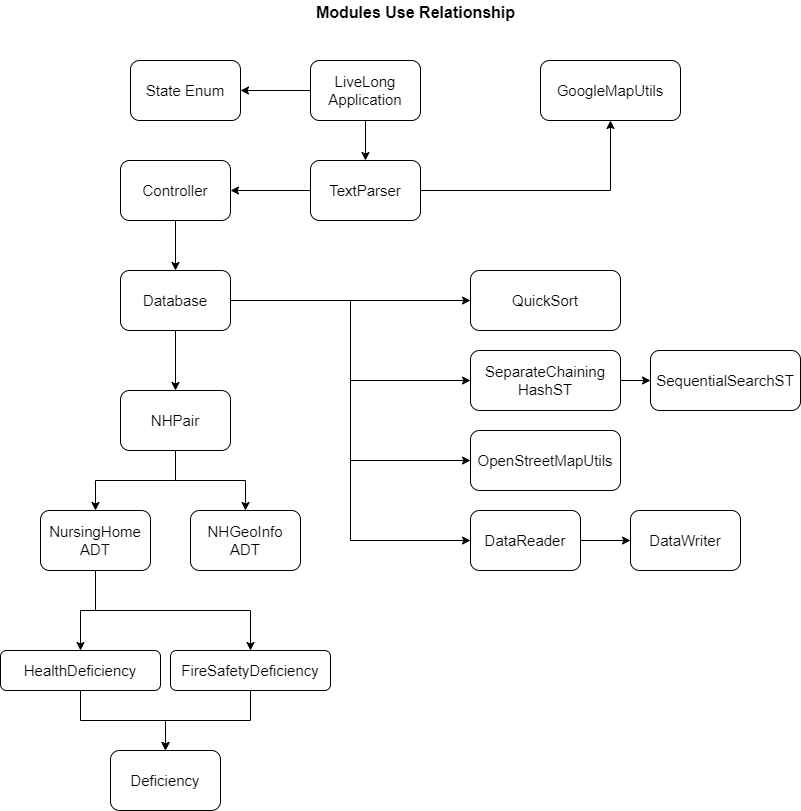
\includegraphics[width=16cm]{Pictures/LiveLong ModulesUsage.png}
\end{center}



%%%%%%%%%%%%%%%%%%%%%%%%%%%%%%%%%%			REQUIREMENTS

\newpage
\section{Tracing Back to Requirements}


\begin{center}
\begin{tabular}{|ll|}
\hline
Functional Requirements & Modules Handling Requirements \\
\hline
NursingHome ADT & \textbf{NursingHome}, \textbf{Deficiency}\\
\hline
NHGeoInfo ADT & \textbf{NHGeoInfo}, \textbf{DataReader}, \textbf{OpenStreetMapUtils}\\
\hline
Generic Deficiency ADT & \textbf{Deficiency},  \textbf{DataReader}\\
\hline
FireSafetyDeficiency ADT & \textbf{FireSafetyDeficiency}, \textbf{Deficiency},  \textbf{DataReader}\\
\hline
HealthDeficiency ADT & \textbf{HealthDeficiency}, \textbf{Deficiency},  \textbf{DataReader}\\
\hline
NHDatabase & \textbf{Database}, \textbf{DataReader}, \textbf{DataWriter}\\
\hline
CSVReader & \textbf{DataReader}, \textbf{DataWriter} \\
\hline
Menu & \textbf{Controller}, \textbf{TextParser}, \textbf{LiveLong}, \textbf{State}\\
\hline
\end{tabular}
\end{center}

\bigskip

\begin{center}
\begin{tabular}{|ll|}
\hline
NF Requirements & Modules Handling Requirements \\
\hline
Reliability & \textbf{Database}, \textbf{DataReader}, \textbf{SequentialChainingHashST}, \textbf{QuickSort}\\
\hline
Accuracy of Results & \textbf{Database}, \textbf{DataReader}, \textbf{SequentialChainingHashST}, \textbf{QuickSort}\\
\hline
Performance & \textbf{DataReader}, \textbf{DataWriter}, \textbf{QuickSort}, \textbf{SequentialChainingHashST}\\
\hline
Usability & \textbf{LiveLong}, \textbf{GoogleMapsUtils}, \textbf{TextParser}, \textbf{Controller}\\
\hline
Scalability &  \textbf{DataReader}, \textbf{DataWriter}, \textbf{QuickSort}, \textbf{SequentialChainingHashST}\\
\hline
\end{tabular}
\end{center}













%%%%%%%%%%%%%%%%%									IMPLEMENTATION DETAILS
\newpage
\section{Implementation Details}
\subsection{classes package}
\subsubsection{NursingHome.java}
An immutable object that is constructed directly from a row in the CSV file. Its variables are all used to store information regarding a Nursing Home in the US Medicare dataset. \\ \\
Additionally, there is a variable that holds a List of Deficiency objects to store FireSafetyDeficiency and HealthDeficiency objects that refer to this NursingHome. There is a method to return the number of active deficiencies in this list. \\ \\
There is a method used to return all values, except for the \textbf{List$<$Deficiency$>$} variable, as a String array. This is used to allow the writing of data into a compressed CSV file that only has the important information, which can then be used to initialize the database faster. \\ \\
Finally, there is a simplified toString() method printing out a summarized version of the values, and a detailed() method returning a string with all the details.

\subsubsection{NHGeoInfo.java}
An object constructed from the dataset pertaining to the geological information of a NursingHome. It contains the \textbf{id}, \textbf{latitude}, and \textbf{longitude} values, which are immutable. The last variable \textit{\textbf{distance}} is calculated using the given lat and long values, and taking another location's values as the target. \\ \\ 
The \textbf{distance} variable is mutable to allow for the application to change the user's location during runtime. \\ \\
There is a method used to return all values as a String array. This is used to allow the writing of data into a compressed CSV file that only has the important information, which can then be used to initialize the database faster.

\subsubsection{NHPair.java}
NHPair is used to create a pair of \textbf{NursingHome} and \textbf{NHGeoInfo} objects that both have the same ID value. Used primarily when returning the results of a search filter, and provides both the values and the geological information of a Nursing Home. Additionally, it allows for a unique sort order such that a list of NHPair is sorted by NursingHome ratings first, then by NHGeoInfo's distance value.

\subsubsection{Deficiency.java}
An immutable object constructed from the datasets referring to either FireSafetyDeficiencies or HealthDeficiencies datasets. Its variables are used to store information parsed from the CSV file. \\ \\
There is a method to check whether this Deficiency is still active based on the Deficiency Status and Status Date. This is used when determining if this deficiency should be shown to the user (I.e. if no longer active, do not show) \\ \\
Finally, there is a method used to return all values as a String array. This is used to allow the writing of data into a compressed CSV file that only has the important information, which can then be used to initialize the database faster. 

\subsubsection{FireSafetyDeficiency and HealthDeficiency.java}
No private entities. Subclasses of Deficiency.java. Only difference between the two is their \textbf{toString()} methods
%%%%%%%%%%%%%
\newpage
\subsection{data package}
\subsubsection{Database}
Contains the following private variables:
\begin{itemize}
\item String \textbf{address} : storing location of the user
\item double \textbf{latitude} : storing latitude value of address
\item double \textbf{longitude} : storing longitude value of address
\item SeparateChainingHashST$<$String, NursingHome$>$ \textbf{stNH}: \\storing NursingHome objects in hash table using NursingHome.getId() as Key. 
\item List$<$NHGeoInfo$>$ \textbf{nhGeo} : storing NHGeoInfo objects as a list. Used for applying QuickSort
\end{itemize}
It contains one private method ``\textbf{updateDistances()}'' to go through all NHGeoInfo objects in \textbf{nhGeo} and prompts them to recalculate their \textbf{distance} variable with the latitude and longitude values. This is called once at initialization, and whenever the database is prompted to change the user's location. \\ \\
Once updated, it does a QuickSort on nhGeo to re-sort the list from lowest distance to highest, so that when answering a search request it needs to simply start from the first index of \textbf{nhGeo}. \\ \\
Before returning the \textbf{results} of a search as a \textbf{List$<$NHPair$>$}, if the search filter requested the results ordered by ratings, it will do a QuickSort on the results list before returning. This then has the list ordered by ratings instead of distance.
\\ \\
Refer to Figure \ref{fig:DatabaseStateUML} for the Database State UML.


\begin{center}
\begin{figure}
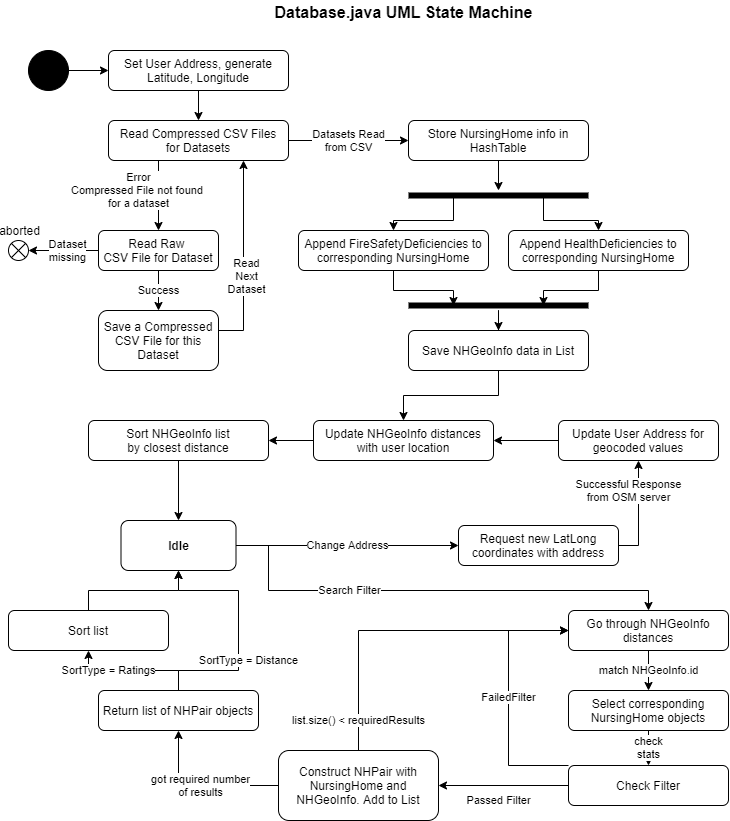
\includegraphics[width=16cm]{Pictures/Database StateMachine.png}
\caption{UML State Machine diagram for \textbf{Database.java}. This class is used to parse and store the information from the dataset CSV files into appropriate data structures. It is constructed with the main goal of being able to provide quick and efficient operations on the data to account for scalability with growing datasets.}
\label{fig:DatabaseStateUML}
\end{figure}
\end{center}

\newpage
\subsubsection{DataReader}
Has private methods to check if a file exists before trying to read. Each public read method has a flow to go through:
\begin{enumerate}
\item Attempt to read compressed CSV file
	\begin{enumerate}
	\item If failed (I.e. File not found), try to read Raw CSV file.
	\end{enumerate}
\item Parse the List$<$String$[]$$>$ from the CSV
\item Construct the object from the String[] and store in a List$<$Object$>$
	\begin{enumerate}
	\item If reading Raw CSV file, use DataWrite to save this List$<$Object$>$ as a compressed CSV version for future use.
	\end{enumerate}
\item Return the List$<$Object$>$. End.
\end{enumerate}
If both the compressed and raw versions of the datasets are not found, throw an exception and stop the application.



\subsubsection{DataWriter}
No private methods. Used to simply write a List$<$String[]$>$ into a CSV file delimited by commas. Generally, this CSV file is a more compressed version of the raw dataset, since it does not include unused columns or empty cells.

%%%%%%%%%%%%%
\newpage
\subsection{app package}
\subsection{LiveLong}
Contains a private \textbf{State} enum variable to control what the user should see and what interaction they can do. \\ \\
Contains a private variable to reference a \textbf{TextParser} object, which it where it sends the user's input in the Command Line along with the current application state. \\ \\
Uses a while loop to continuously wait for a user's input to send to the TextParser. Until the application state is changed to Exiting, this application loop will repeat. \\ \\
The \textbf{setAppState(State)} and \textbf{getAppState()} are `static', such that they can be accessed from other classes. \\ \\
Upon using \textbf{setAppState(State)}, tell \textbf{TextParser} to print the screen corresponding to the current State
\\ \\
Refer to Figure \ref{fig:LiveLongStateUML} for a LiveLong Application State UML.

\begin{center}
\begin{figure}
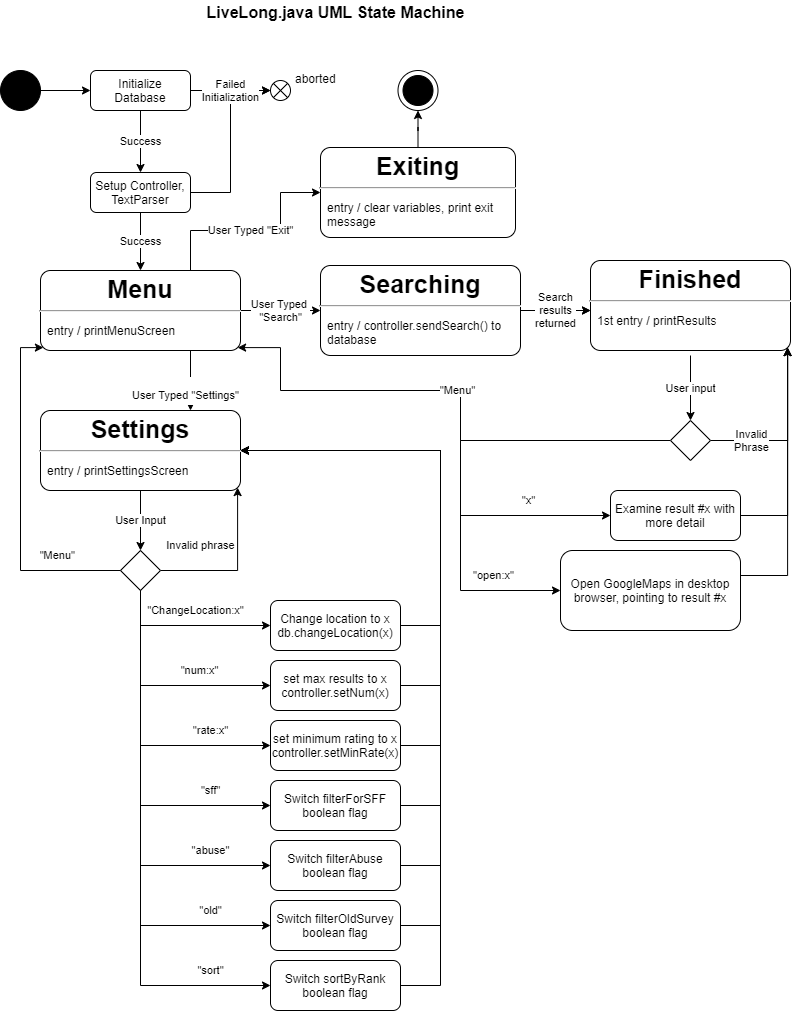
\includegraphics[height=18cm]{Pictures/LiveLong StateMachine.png}
\caption{UML State Machine diagram for \textbf{LiveLong.java}. This class runs the application loop and interacts with the command line interface to retrieve results from the database. Responses received in the CLI from the user is parsed into appropriate commands, and visual feedback is provided to the user on the current state of the application.}
\label{fig:LiveLongStateUML}
\end{figure}
\end{center}

\newpage
\subsubsection{Controller}
Has the following private variables
\begin{itemize}
\item Database \textbf{db} : reference to the \textbf{Database} to request information from
\item List$<$NHPair$>$ \textbf{results} : results retrieved from \textbf{Database.search()}
\item int \textbf{numResults} : storing longitude value of address
\item int \textbf{minRating} : storing longitude value of address
\item boolean \textbf{filterForSFF} : Search Filter - show only NH's that are SFF or is an SFF candidate
\item boolean \textbf{filterAbuse} : Search Filter - show only NH's that have had no history of abuse
\item boolean \textbf{filterOldSurvey} : Search Filter - show only NH's that have been inspected recently ($<$ 2 years)
\item boolean \textbf{sortByRank} : Search Filter - how the \textbf{results} should be sorted
\end{itemize}
When using \textbf{sendSearch()}, \textbf{Database.search()}, the returned  List$<$NHPair$>$ is stored in \textbf{results}. After receiving the results, use \textbf{LiveLong.setAppState(State.Finished)} to notify the application that the results have been received.


\newpage
\subsubsection{TextParser}
Has the following private methods that each correspond to the given State. The public methods \textbf{receive(String, State)} and \textbf{ printScreen(State)}, depending on the given State, call the corresponding methods.
\begin{itemize}
\item void \textbf{printScreen(State)} :
\begin{enumerate}
	\item State.Menu $\Rightarrow$ \textbf{printMenu()}
	\item State.Settings $\Rightarrow$ \textbf{printSettings()}
	\item State.Finished $\Rightarrow$ \textbf{printFinished()}
	\item State.Exiting $\Rightarrow$ \textbf{printExiting()}
\end{enumerate}
\item void \textbf{receive(String,State)} :
\begin{enumerate}
	\item State.Menu $\Rightarrow$ \textbf{handleMenuResponse(String)} 
		\begin{itemize}
		\item ``Search'' $\Rightarrow$ \textbf{LiveLong.setAppState(State.Searching)}, \\ prompt \textbf{controller.sendSearch()}
		\item ``Settings'' $\Rightarrow$ \textbf{LiveLong.setAppState(State.Settings)}
		\item ``Exit'' $\Rightarrow$ \textbf{LiveLong.setAppState(State.Exiting)}
		\end{itemize}
	\item State.Settings $\Rightarrow$ \textbf{handleSettingsResponse(String)}
		\begin{itemize}
		\item ``ChangeLocation:x'' $\Rightarrow$ \textbf{controller.requestChangeLocation(x)}
		\item ``num:x'' $\Rightarrow$ \textbf{controller.setNumResults(x)}
		\item ``rate:x'' $\Rightarrow$ \textbf{controller.setMinRating(x)}
		\item ``sff'' $\Rightarrow$ Swap Controller.isFilterForSFF
		\item ``abuse'' $\Rightarrow$ Swap Controller.isFilterAbuse
		\item ``old'' $\Rightarrow$ Swap Controller.isFilterOldSurvey
		\item ``sort'' $\Rightarrow$ Swap Controller.isSortByRank
		\item ``Menu'' $\Rightarrow$ \textbf{LiveLong.setAppState(State.Menu)}
		\end{itemize}
	\item State.Finished $\Rightarrow$ \textbf{handleFinished(String)}
		\begin{itemize}
		\item ``x'' $\Rightarrow$ Print out the NursingHome object at index x of \textbf{controller.getResults()} with more details
		\item ``open:x'' $\Rightarrow$ Open in GoogleMaps the user's location and the target NursingHome object at index x of \textbf{controller.getResults()} 
		\item ``Menu'' $\Rightarrow$ \textbf{LiveLong.setAppState(State.Menu)}
		\end{itemize}
\end{enumerate}
\end{itemize}
If a state is not mentioned, then there is no method called.

\newpage
\subsection{util package}
\subsubsection{GoogleMapUtils}
A singleton instance, available for any class in application to call. Opens GoogleMaps given a starting and destination address. The given addresses are URL-escaped to be able to be put in the browser URL field. It builds the website/query name with the provided addresses, then prompts the Desktop to open the constructed URL in the default browser.

\subsubsection{OpenStreetMapUtils}
A singleton instance. Requests geocoding on a string, usually an address. Builds a query to the OpenStreetMap website with the address. A response is received in JSON format. Only the latitude and longitude values are currently saved. Values are saved in a Map, with key ``lat'' and ``lon''. If no response is received, returns null.


\subsubsection{QuickSort}
An implementation of the QuickSort algorithm. Code is directly pulled from the Algorithms 4th Edition textbook used in CS2XB3.

\subsubsection{SeparateChainingHashST}
An implementation of a Hash symbol table using chaining. Code is directly pulled from the Algorithms 4th Edition textbook used in CS2XB3, and from Lab 9.

\subsubsection{SequentialSearchST}
An implementation of a symbol table linked list. Code is directly pulled from the Algorithms 4th Edition textbook used in CS2XB3, , and from Lab 9.



\newpage
\section{Internal Review}
$LiveLong$ has accomplished its main goal of being able to quickly deliver information about nearby nursing homes to a client. Clients are able to change their location during runtime, and are also able to modify their search filters to get information that is more relevant to their needs. Results also clearly show any warnings that a establishment may have, from ranging to past complaints and penalties, to official warnings and inspections carried out by the government.
\\ \\
With the current iteration, initialization of the application takes less than 10 seconds maximum to parse through four datasets totaling over 500,000 rows of information. Additionally, a compressed version of the datasets is saved locally after the first initialization, allowing for faster load times when launching the app again.
\\ \\
The search functionality also returns results very quickly, making user interaction with the application responsive with little wait times.
\\ \\
The only interaction with the application that results in a longer wait would be changing the user's location, since the application has to request a geocoding process and response from an online service. In this case, that third party service is the only limiting factor in the speed of the application. Even then, the requests usually last three to five seconds maximum, depending on the current traffic load.
\\ \\
In regards to the Requirements Specification document, LiveLong has met most of the requirements. Performance-wise, LiveLong has become a very fast application and delivers results back almost instantaneously. It accurately and reliably returns the expected results each time, and can handle unexpected inputs from the user.
\\ \\
With its good performance and reliability, LiveLong is likely able handle future scalability very well. A doubling in size of the datasets only really affect the initialization times, and not the actual user interactions with the database. The only downside is that newly updated datasets have to be downloaded and manually placed in a location that LiveLong can reach, involving some human interference instead of being a stand-alone application of itself.
\\ \\
Finally, LiveLong was designed with a MVC design pattern and with modularity in mind. This means that it would be simple to implement a new UI interface, or to change the internal implementation of a class (I.e. algorithms, data structures, etc.). Thus, LiveLong can most likely handle future changes with minimal problems.
\\ \\
In short, LiveLong has completed what it set out to do: to deliver important information from official datasets about Nursing Homes to the client in a quick and efficient manner. It is capable of handling many different situations (I.e. changing locations, changing search filters, increased datasets size) and accurately reporting the results back to the client. The speed and efficiency it demonstrates proves that it would be able to handle scalability with larger datasets in the future, and its modular nature allows additions and modifications to its components to be simple and easy to implement. Its weaknesses is mainly in how retrieving updated datasets requires the downloading and movement of a file to a proper folder.
\end {document}